\chapter{Extração e Transformação}

Como referido no capítulo anterior, para realização da extração e transformação dos dados para análise estatística foram utilizadas as plataformas \textbf{\textit{KNIME}} e \textbf{\textit{SPOON}}. Cada um dos elementos do grupo fez uso de uma das ferramentas para realização do mesmo processo.

Assim sendo, passaremos à explicação das solução para cada uma das ferramentas utilizadas.

\section*{KNIME}
A solução desenvolvida em \textbf{\textit{KNIME}} é constituída por 4 passos principais:
\begin{itemize}
    \item Obtenção os dados da API.
    \item Transformação dos dados de forma relevante (dados estatísticos).
    \item Formatação dos dados em \textbf{JSON, XML e CSV}.
    \item Envio dos dados para Email.
    \item Repetição do Processo.
\end{itemize}

\subsection*{Obtenção dos Dados da API}

Na API do IPMA encontram-se disponíveis dados no formato \textbf{CSV} relativos a \textbf{Temperaturas Máximas}, \textbf{Temperaturas Mínimas} e \textbf{Dados de Precipitação}. Estes ficheiros encontram-se separados por Concelho o que faz com que seja necessário o acesso ao ficheiro referente a cada concelho individualmente. 

Ainda na mesma API estão presentes ficheiros \textbf{JSON} referentes à \textbf{Previsão do Tempo nos próximos 5 dias}, assim como os ficheiros CSV estes encontram-se separados, neste caso não por concelho mas por Distrito. 

Como todos os ficheiros se encontram separados foram criados 4 \textit{workflows}, um para cada tipo de dados necessários, temperaturas máximas e mínimas, precipitação e ainda previsão do tempo.

Para cada um dos concelhos foi necessário utilizar um nodo de leitura de CSV para obtenção dos dados, assim como associada a cada tabela uma coluna extra com o nome de cada local, para ser mais facilmente identificado assim que todos os dados fossem juntos na mesma tabela.

\begin{figure}[H]
    \centering
    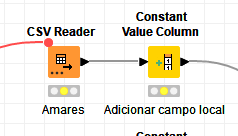
\includegraphics{imagens/nodoBuscaCsv.png}
    \caption{Processo de Obtenção de Dados}
\end{figure}


Como para o Distrito de Braga existem 14 Concelhos. seriam necessários 14 nodos para obter os dados referentes a cada um.

Para cada um dos dados necessários, Temperaturas Máximas e Mínimas e Precipitação a API fornece ficheiro CSV nos seguintes formatos:

\newpage
\title{\textbf{Precipitação Total}}


\begin{figure}[H]
    \centering
    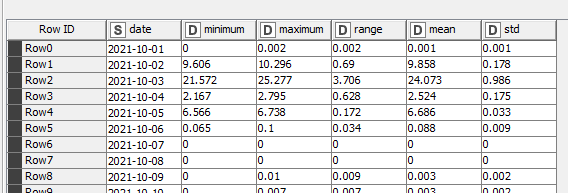
\includegraphics[scale=0.7]{imagens/PrecipitaFormatIPMA.png}
    \caption{Formato dos dados de Precipitação do IPMA}
\end{figure}

\title{\textbf{Temperatura Máxima}}

\begin{figure}[H]
    \centering
    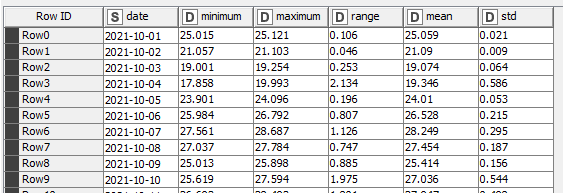
\includegraphics[scale=0.7]{imagens/TempMaxFormatIPMA.png}
    \caption{Formato dos dados de Temperatura Máxima do IPMA}
\end{figure}


\textbf{Temperatura Mínima}

\begin{figure}[H]
    \centering
    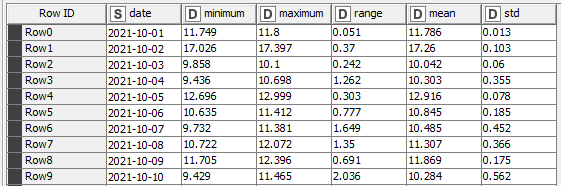
\includegraphics[scale=0.7]{imagens/TempMinFormatIPMA.png}
    \caption{Formato dos dados de Temperatura Mínima do IPMA}
\end{figure}

\newpage

\textbf{Previsão do Tempo}

No entanto, para os dados de previsão do tempo a API fornece dados no formato JSON, dados estes que são convertidos em tabela para serem mais facilmente manuseados, o formato é o seguinte:


\begin{figure}[H]
    \centering
    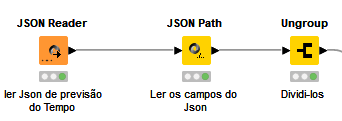
\includegraphics[]{imagens/PrevJsonFormatReader.png}
    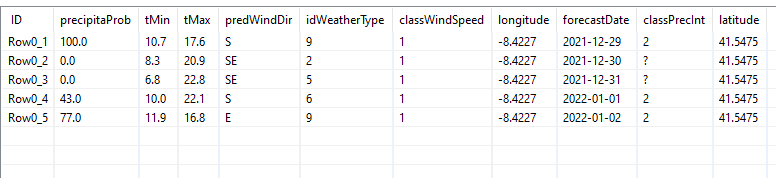
\includegraphics[scale=0.6]{imagens/PrevFormatIPMA.png}
    \caption{Formato dos dados de Previsão do tempo do IPMA}
\end{figure}

Para cada uma das tabelas acima, à exceção da previsão do tempo, era ne\-cessário adicionar um campo que identificasse o local de onde eram provenientes os da\-dos, pois como os ficheiros se encontravam separados esta identificação não existia.

Desta forma, foi adicionada a cada tabela de dados a coluna \textbf{"local"} para melhor identificar os dados para análise.

O formato de todas as tabelas seria semelhante a este:

\begin{figure}[H]
    \centering
    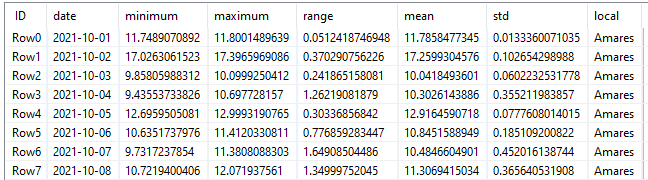
\includegraphics[scale=0.7]{imagens/localFormat.png}
    \caption{Formato dos dados depois de ser adicionado o campo local}
\end{figure}

\subsection*{Transformação dos dados de forma relevante}

Após a agregação dos dados em tabelas, seria necessário efetuar as devidas transformações de modo a obter os dados estatísticos relevantes. Para cada um dos \textit{workflows} existem transformações semelhantes de forma a apresentar os dados organizados. 

No entanto existem algumas diferenças entre eles, fazendo assim com que seja necessário que sejam apresentados individualmente, principalmente nos dados referentes às previsões do tempo.

\subsubsection*{Temperatura Máxima/Mínima e Precipitação}

O formato genérico para as transformações do \textit{workflow} das \textbf{temperaturas e de precipitação} é o seguinte:

\begin{figure}[H]
    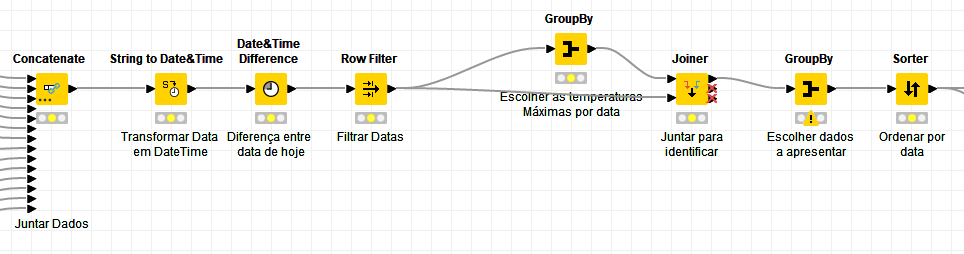
\includegraphics[scale=0.5]{imagens/TranformationGenericFormat.png}
    \caption{Transformações Temperaturas Máxima/Mínima e Precipitação}
\end{figure}

Após todas as tabelas serem concatenadas no nodo \textbf{Concatenate} é calculada a diferença entre a data referente ao dia presente na tabela com o dia atual com o nodo \textbf{Date\&Time Difference}, este valor é associado a uma coluna que é adicionada à tabela com o nome \textbf{"diff"}. 

Como apenas queremos apresentar os dados referentes aos \textbf{últimos 10 dias} são filtrados os dados cuja diferença seja maior do que 10 através do nodo \textbf{Row Filter}

\begin{figure}[H]
    \centering
    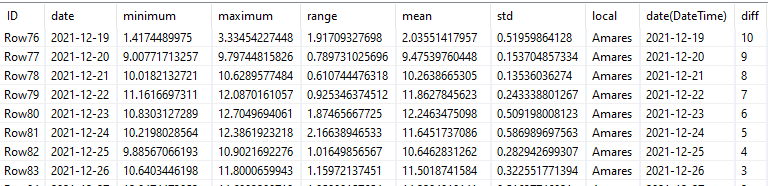
\includegraphics[scale=0.65]{imagens/tablediff.png}
    \caption{Tabela com a coluna "diff" associada}
\end{figure}


Depois de filtrados os dados são organizados pelo valor que nós queremos obter por cada data através do nodo \textbf{Group By}. 

Este nodo organiza os dados por data, e faz a sua agregação mediante um valor, no caso da figura acima agrega os dados pela maior temperatura encontrada com uma data associada

\begin{figure}[H]
    \centering
    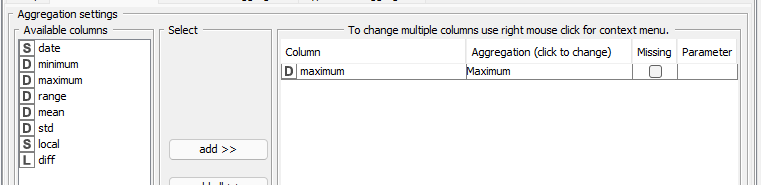
\includegraphics[scale=0.67]{imagens/maiortemperaturaGroupBY.png}
    \caption{Agregação valor máximo de temperatura}
\end{figure}

\begin{figure}[H]
    \centering
    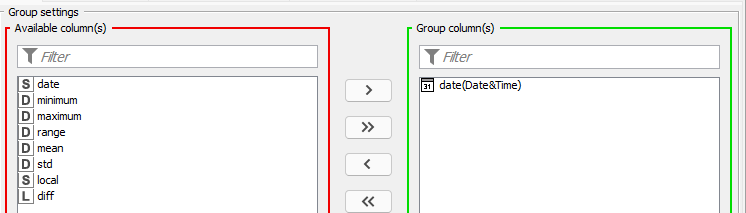
\includegraphics[scale=0.67]{imagens/dataGroupBY.png}
    \caption{Organização por Data}
\end{figure}


Depois de organizados, os dados são ordenados por data através do nodo \textbf{Sorter}

Este processo é repetido nos 3 processos (Temperatura Máxima/Mínima e Precipitação), no entanto, no processo de temperatura mínima, os dados ao invés de organizados pelo maior valor, são organizados pelo menor.

\subsubsection*{Previsão do Tempo}

Para o processo de transformação de dados de previsão do tempo, o \textit{workflow} ocorre de forma diferente.

O formato dos dados de previsão do tempo inclui diversos \textbf{ID} para dados dos quais não temos acesso direto, para termos acesso a tais dados temos de associar os \textbf{ID} a tabelas presentes na API com esse propósito.

O tipo de dados dos quais não temos acesso são: \textbf{Classe de Precipitação}, \textbf{Classe da velocidade do Vento} e ainda o \textbf{Tipo de Clima}.

A tabela sem qualquer tipo de transformações encontra-se da seguinte forma:

\begin{figure}[H]
    \centering
    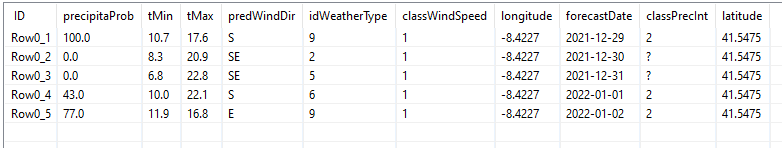
\includegraphics[scale=0.65]{imagens/prevNotransTable.png}
    \caption{Tabela de Previsão do Tempo sem transformações}
\end{figure}

As tabelas às quais temos de associar a tabela inicial, com dados referentes ao tipo de clima, precipitação e velocidade do vento são as seguintes:


\begin{figure}[H]
    \centering
    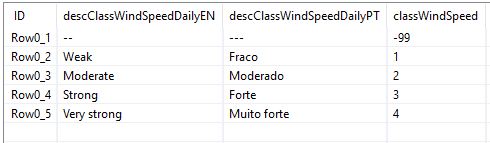
\includegraphics[]{imagens/WindType.png}
    \caption{Tabelas de descrição da velocidade do Vento}
\end{figure}

\begin{figure}[H]
    \centering
    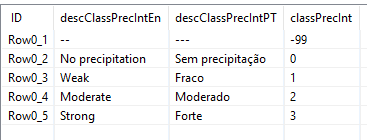
\includegraphics[]{imagens/PrecType.png}
    \caption{Tabela de descrição de Precipitação}
\end{figure}

\begin{figure}[H]
    \centering
    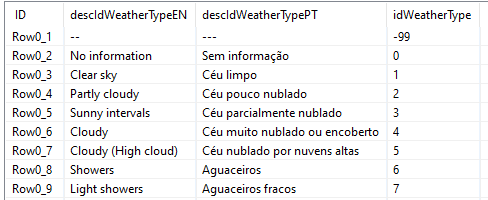
\includegraphics[]{imagens/WeatherType.png}
    \caption{Tabela de descrição do Clima}
\end{figure}

\newpage

Para cada uma destas tabelas está associado um nodo \textbf{Joiner} para juntar as duas tabelas através do \textbf{ID} correspondente, assim como um \textbf{Column Filter} para remover as colunas não desejadas.

O \textit{workflow} procede da seguinte forma:

\begin{figure}[H]
    \centering
    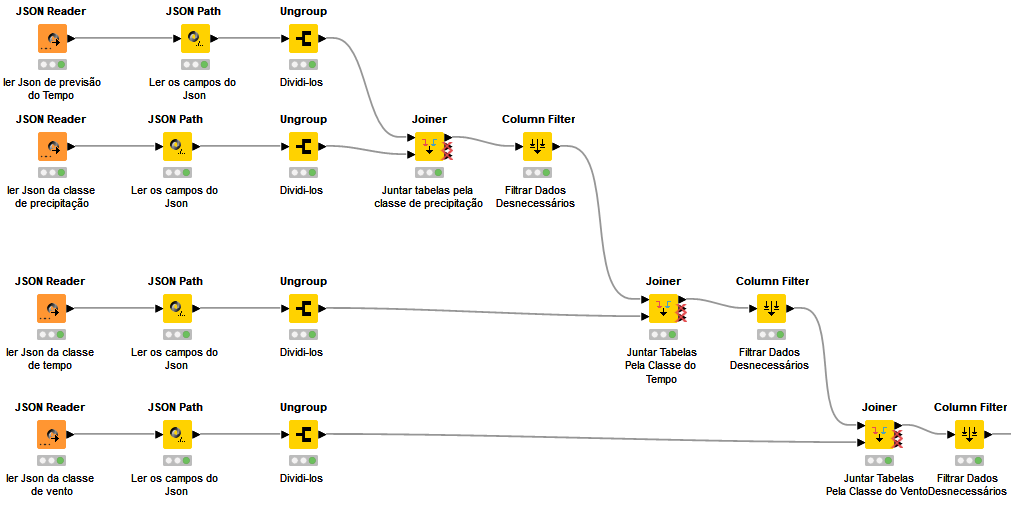
\includegraphics[scale=0.5]{imagens/prevWorkflowTrans.png}
    \caption{Transformações no workflow de previsão de Tempo}
\end{figure}

Os dados depois de todas as transformações geram uma tabela com o seguinte formato:

\begin{figure}[H]
    \centering
    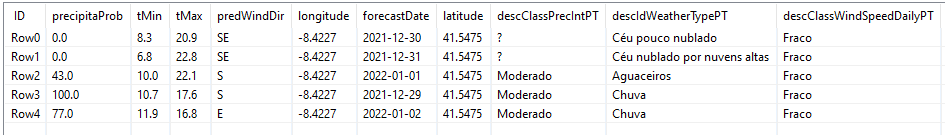
\includegraphics[scale=0.6]{imagens/TabelaFinalPrev.png}
    \caption{Tabela final de previsão do tempo}
\end{figure}

\newpage

\subsection*{Formatação dos dados em JSON, XML e CSV}
Depois do processo anterior é necessário, para cada um dos \textit{workflows}, guardar os dados em diversos formatos de ficheiro, neste caso \textbf{JSON}, \textbf{XML} e \textbf{CSV}.

Para esse efeito foram utilizados os mesmos nodos para transformação nos 3 formatos:

\begin{figure}[H]
    \centering
    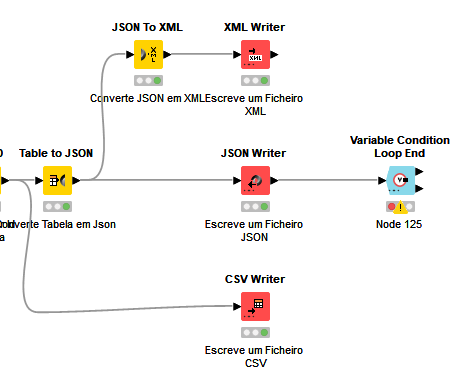
\includegraphics[scale=0.7]{imagens/FileTrans.png}
\end{figure}

Estes nodos utilizam os dados provenientes das tabelas e guardam ficheiros nas pastas XML, CSV e JSON.

Estes ficheiros podem ser acedidos posteriormente para os processos de apresentação de dados (Email, Dashboard, Discord API).

\newpage
\subsection*{Envio de Dados para Email}

Uma das formas de apresentação dos dados é através do envio diário de um email com as tabelas referentes aos dados relevantes.

Para o envio do email é necessário que o \textbf{KNIME} faça o processamento das tabelas de forma a serem legíveis por parte do recipiente.

\subsubsection{Formatação das Tabelas}

\begin{figure}[H]
    \centering
    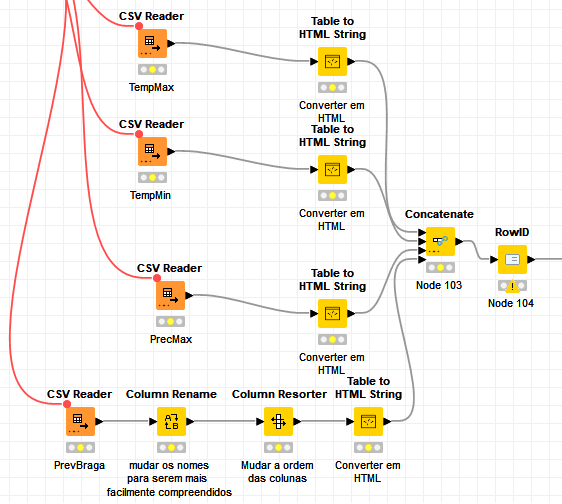
\includegraphics[scale=0.7]{imagens/sendemailgetdata.png}
    \caption{Formatação de dados para email}
\end{figure}

Para as tabelas serem legíveis por parte do recipiente é necessário fazer a formatação para \textbf{HTML}, para isso é o utilizado o nodo \textbf{Table to HTML string} que trata de tal formatação. A tabela de previsões no entanto tem dois nodos extra que servem para renomear as colunas para serem mais facilmente compreendidas e ainda a sua reordenação para o mesmo efeito.

Depois de convertidas para \textbf{HTML} as tabelas são juntas para poderem ser enviadas como variáveis no email.

\subsubsection{Envio de email}

\begin{figure}[H]
    \centering
    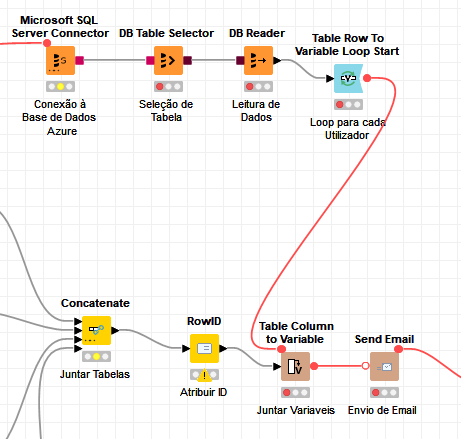
\includegraphics{imagens/SendemailSendEmail.png}
    \caption{Envio de email}
\end{figure}

Para proceder ao envio dos emails para os utilizadores, o \textbf{KNIME} tem de aceder primeiro à base de dados \textbf{Azure} que definimos, esta base de dados encontra-se no servidor "isitp2tempo.database.windows.net". Nesta base de dados temos os utilizadores para os quais enviaremos emails.

\newpage
Os dados presentes na base de dados são os seguintes:

\begin{figure}[H]
    \centering
    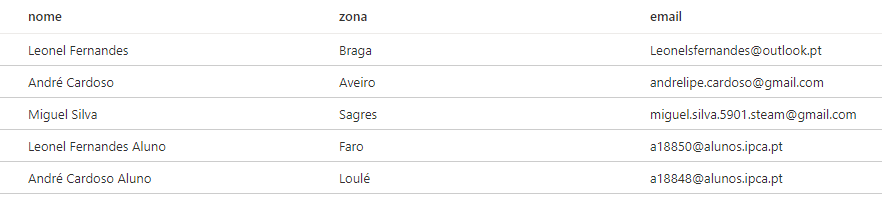
\includegraphics[scale=0.6]{imagens/Users.png}
    \caption{Lista de utilizadores para envio de email}
\end{figure}

Após obter os utilizadores o nodo \textbf{Table Row To Variable Loop Start} vai repetir o processo de envio para cada um dos presentes na tabela.

A escolha de destinatário também é definida através da variável \textbf{email} presente na tabela.

Quando o processo estiver concluído todos os utilizadores receberão um email com as tabelas dos dados
meteorológicos proveniente do email "weather.isitp2\-@outlook.pt".

\newpage
\subsection*{Repetição do Processo}

Todos os processos referidos até agora necessitam ser automatizados para terem algum tipo de utilidade,
como tal, foram utilizados nodos disponibilizados na plata\-forma \textbf{KNIME} para criar repetição 
de todos os processos definindo um intervalo de tempo.

\begin{figure}[H]
    \centering
    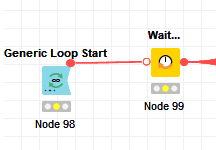
\includegraphics[]{imagens/Loop.png}
    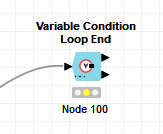
\includegraphics[]{imagens/LoopEND.png}
    \caption{Processo de Loop}
\end{figure}


Para a \textbf{obtenção dos dados} foi definido o intervalo de tempo de 1 hora entre cada request dos ficheiros CSV para a API do IPMA, isto é feito para manter os dados atualizados.

Já para o processo de \textbf{envio de email} foi definido o intervalo de tempo de 24 horas entre cada iteração do programa.





